\documentclass[a0,final]{a0poster}
%%%Load packages
\usepackage{multicol} 			%3-column layout
\usepackage[left=2cm,right=2cm,bottom=0cm,top=0cm]{geometry}			%Reset margins
\usepackage[T1]{fontenc}			%Need for gtamac fonts
\usepackage{textcomp}
\usepackage{mathpazo}			%Load palatino font & pazo math
\usepackage{graphicx}
\usepackage[a4paper, total={36in, 42in}]{geometry}
%%% modified by Karol Kozioł for ShareLaTeX use
%\usepackage{gtamacdidot}		%Set serif to Didot & sans to Optima
%\usepackage{color}				%Needed for colour boxes & coloured text

\usepackage{xcolor}
\usepackage{tgtermes} % serif font
\usepackage{tgheros} % sans font
\usepackage{caption}
\usepackage{array}
\usepackage{tabularx}
\setlength\extrarowheight{8pt}
%%%


%%%Define colours and lengths
\definecolor{headingcol}{rgb}{1,0.7,0}		%Colour of main title
\definecolor{fillcol}{rgb}{0.8,0.8,1}			%Fill-colour of box
\definecolor{boxcol}{rgb}{0.1,0.1,0.4}		%Edge-colour of box and top banner
\fboxsep=1cm							%Padding between box and text
\fboxrule=2mm							%Width of box outline
\renewcommand{\rmdefault}{ppl}			%Reset serif to Palatino
\setlength{\columnsep}{2cm}				%Set spacing between columns
%Uncomment for lines as column separators:
%\setlength{\columnseprule}{1pt}


%%%Format title
\makeatletter							%Needed to include code in main file
\renewcommand\@maketitle{%
\null									%Sets position marker
{
\color{headingcol}\sffamily\VERYHuge		%Set title font and colour
\@title \par}%
\vskip 0.6em%
{
\color{white}\sffamily\large				%Set author font and colour
\lineskip .5em%
\begin{tabular}[t]{l}%
\@author
\end{tabular}\par}%
\vskip 1cm
\par
}
\makeatother

\newsavebox\envbox 					%Define name for boxes used

%%%Define "Section" environment for framed boxes
%%%Usage: \begin{Section}{Name} blah blah blah \end{Section}
\newenvironment{Section}[1]				%Environment takes one argument
%%%Opening
{
\par 
\flushleft
\colorbox{boxcol}{% 						%Draws solid colour box around title
\sffamily\large\color{headingcol}> \color{white} #1%Typesets section name
\hspace{0.5cm}}
\par\nobreak 
\nointerlineskip 						%Fits title snugly above box (no gap)
\setlength\parskip{-1pt}					%Even snugger
\begin{lrbox}\envbox						%Opens box environment
\begin{minipage}{0.95\columnwidth}		%Opens minipage environment for section contents
}
%%%Closing
{\par
\end{minipage}\end{lrbox}				%Close minipage and box
\fcolorbox{boxcol}{fillcol}{\usebox\envbox}	%Draw box with contents frame colour: boxcol, fill colour: fillcol
\vspace{1cm}							%Add spacing below box
} 



%---------------------------------------------------------------------------------------------------%
%---------------------------------------------------------------------------------------------------%
%---------------------------------------------------------------------------------------------------%
%---------------------------------------------------------------------------------------------------%
%---------------------------------------------------------------------------------------------------%
%---------------------------------------------------------------------------------------------------%


\title{NYC Real Estate Price Prediction}
\author{Benjamin Jakubowski, Haonan Zhou}
\begin{document}

\hspace{-3cm}								%Align with edge of page, not margin
\colorbox{boxcol}{							%Coloured banner across top
\begin{minipage}{1189mm}					%Minipage for title contents
%\vspace{-13cm}							%Shift up over header image
\maketitle
\end{minipage}}
\vspace{1cm}

\begin{multicols}{3}							%Use 3-column layout
\raggedcolumns							%Don't stretch contents vertically

%%%Column1
\begin{Section}{Introduction}
\subsection*{Problem}
\begin{itemize}
\item In real estate markets, prospective buyers and sellers must valuate properties to inform their asking and offering prices.
\item To do so, many buyers and sellers rely on real estate agents' comparative market analyses, which valuate real estate using past sale prices for comparable properties.
\item We aimed to develop a price prediction model using machine learning algorithms instead of expert intuition and a priori definitions of comparability.
\end{itemize}
\subsection*{Objective}
\begin{itemize}
\item In our modeling, we aimed to minimize median absolute percent error in predicted price. This objective was selected as it is used by the real estate website Zillow to evaluate the accuracy of their price predictions, and thus can be viewed as the industry standard evaluation metric.
\end{itemize}
\end{Section}
\noindent \par
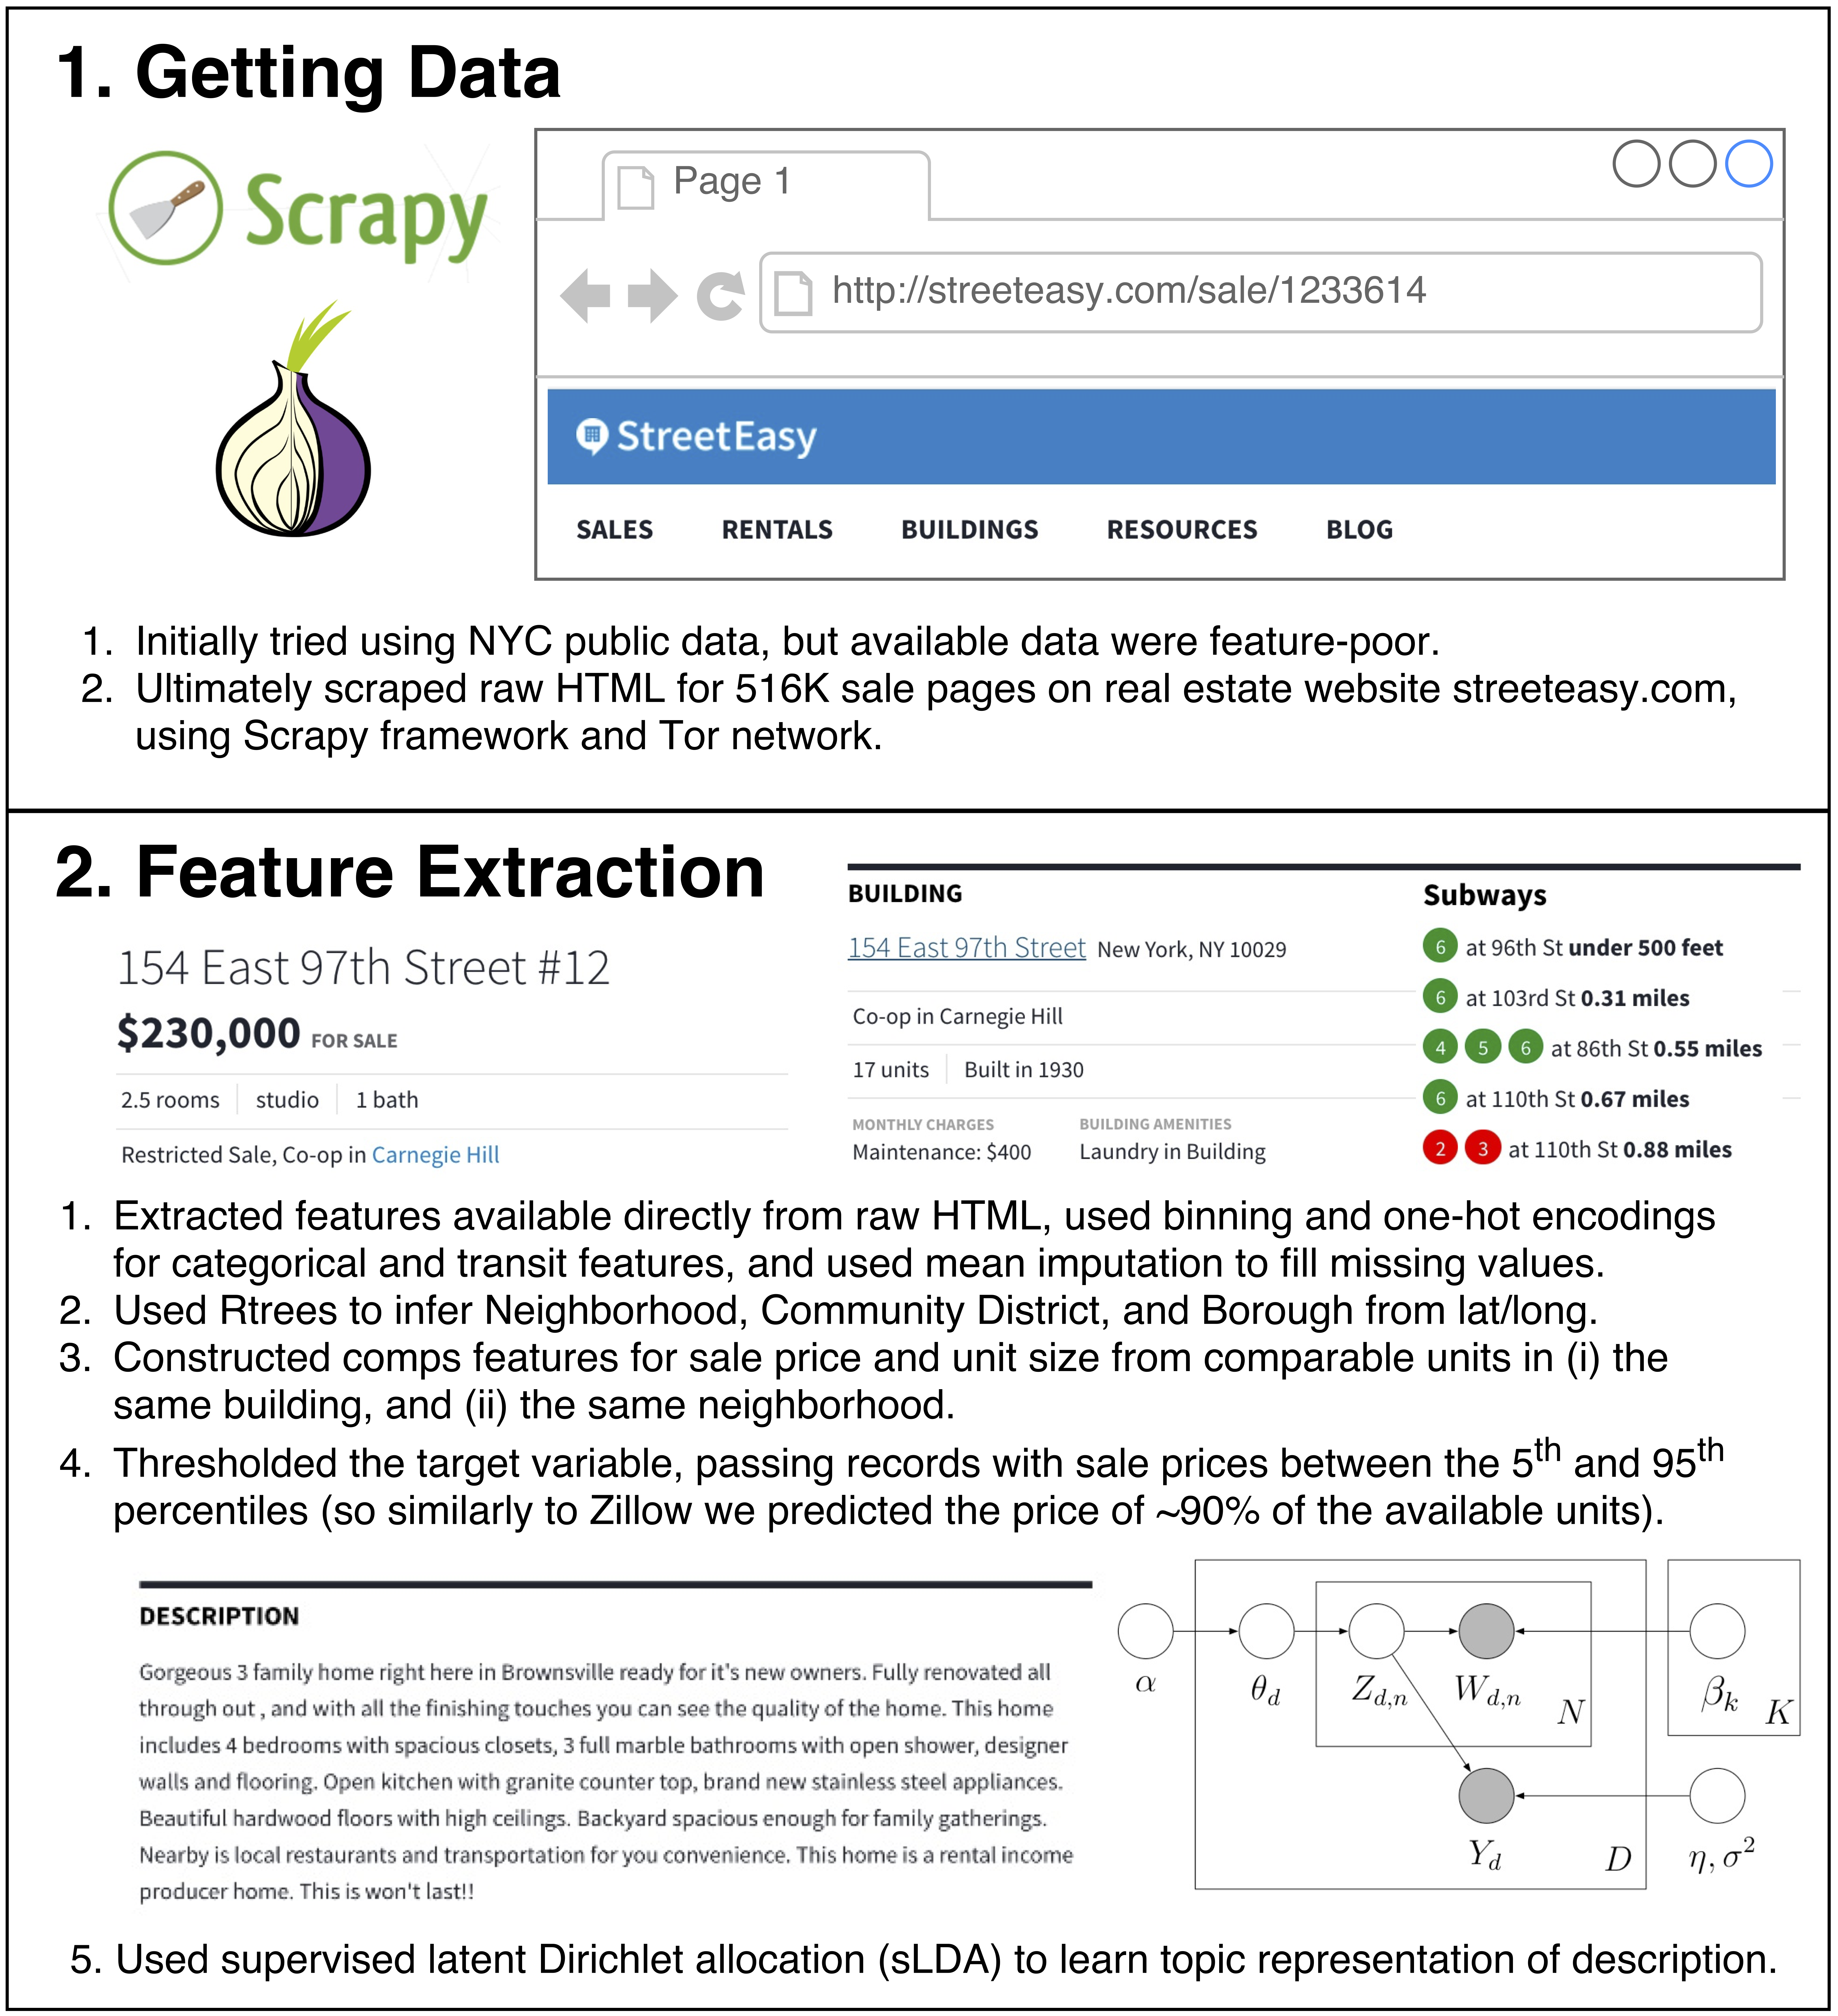
\includegraphics[scale=1.74]{work_flow.png}

\columnbreak
%%%Column2

\begin{Section}{sLDA Featurization}
In streeteasy, much of the information regarding the property type (ex: luxury apartment, pre-war building near the park) is provided by a descriptive paragraph. Hypothesizing these latent style variables could be identified using LDA or sLDA, we learned a number of topic models. These models are summarized in the figures below:
\begin{itemize}
    \item \textbf{Top right}: Learning the optimal $K$ for sLDA and LDA topic models based on validation set log(price) MSE.
    \item \textbf{Bottom right}: Maps of neighborhood median topic weights reveal geographic coherency of learned topics. This example map shows geographic distribution of Topic 7: designed loft properties.
    \item \textbf{Left}: Coefficients learned in the sLDA model can be interpret as the predicted log(price) for the corresponding single topic (one-hot) vector.
\end{itemize}
\end{Section}

\noindent \par

\includegraphics[scale=1.51]{lda_figs_combined.png}

\vspace*{1.1cm}

\begin{Section}{Price Prediction Models}
Following featurization, we tried the following approaches to predictive modeling:
\begin{itemize}
\item \textbf{Linear Models}: We tested linear models for city-wide, borough-level, and community-district level price prediction.
\item \textbf{Non-linear Models}: We tested non-linear models (random forest and additive regression trees using XGBoost) for city-wide price prediction.
\end{itemize}
For the regression problem we initially trained our model with normalized price as the target variable. However as we delved deeper into model optimization, we found that using normalized log price as the target yielded the best validation set performance. Additionally, based on initial hyper-parameter optimization, it was clear XGBoost provided the best performance, so subsequent optimization efforts were focused on tuning XGBoost.
\end{Section}


\columnbreak
%%%Column 3
\begin{Section}{Model Tuning}
Since XGBoost outperform other models in initial experiments, the focus of model tuning was optimizing XGBoost parameters. Experiments included testing:
\begin{itemize}
\item \textbf{Loss functions}: (i) RMSE, (ii) Root Mean Squared Percent Error (RMSPE)
\item \textbf{Target transformations}: (i) Scaled, (ii) log-transformed and normalized. 
\item \textbf{Learning rate}: Grid search over [0.01,0.1,0.3,0.7]
\item \textbf{Max tree depth}: Grid search over [4,6,8,10]
\end{itemize}
First tree depth was optimized, then learning rate and number of rounds of boosting. Loss functions and transformations were tested within this grid search framework.
\end{Section}

\noindent \par
\includegraphics[scale=1.94]{XGBoost_fig.png}

\vspace*{1.1cm}

\begin{Section}{Conclusion}
\begin{itemize}

\item We achieved test set performance comparable to the deployed NYC "Zestimate" model.
\item XGBoost performed best for this problem, compared to random forests and regularized linear models. This is most likely due to its ability learn complex non-linear interactions between the different features we engineered.
\end{itemize}
\end{Section}


\end{multicols}
\end{document}
